\section{Funzionamento del fotovoltaico ibrido}\subsection{Ibrido: polimeri coniugati e nanoparticelle inorganiche}

%%%%%%%%%%%%%%%%%%%%%%%%%%%%%%%%%%%%%%%%%%%%%%%%%%%%%%%%%%%%%%%%%%%%%%%%%%%%%%%%%%%%%%%%%%%%%%%%%%%%%%%%%%%%%%%%%%%%%%%%%%%%%%%%%%%%

\begin{frame}
  \frametitle{Ibrido: polimeri coniugati e nanoparticelle inorganiche}

\begin{description}
 \item[Cella fotovoltaica ibrida:]{modulo fotovoltaico avente \alert{strato fotoattivo} composto sia di materiale organico che inorganico.}
\end{description}

\begin{columns}
\column{0.7\linewidth}
\begin{center}
  \begin{minipage}{6.7cm}  


 \uncover<2->{
\begin{block}{In questo lavoro di tesi:}
\begin{itemize}
 \item materiale organico: \\\alert{poli(3-esiltiofene) regioregolare \\terminato asimmetricamente},
 \item materiale inorganico: \\\alert{nanoparticelle di CdSe}.
\end{itemize}
Entrambi i materiali sono \alert{semiconduttori}.
\end{block}}\end{minipage}
\end{center}\column{0.3\linewidth}

\begin{figure}
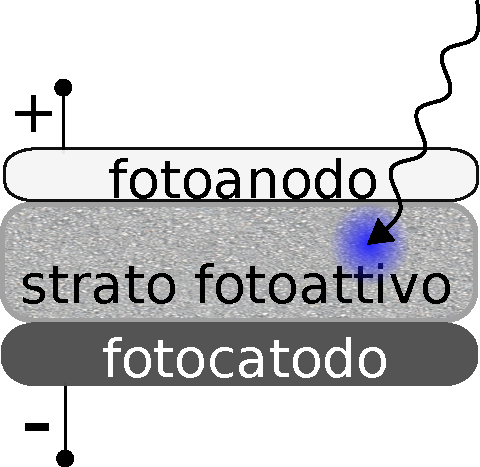
\includegraphics[width=0.9\textwidth]{Immagini_Tesi/pv-schema2.pdf}
\end{figure}
\end{columns}
\end{frame}

%%%%%%%%%%%%%%%%%%%%%%%%%%%%%%%%%%%%%%%%%%%%%%%%%%%%%%%%%%%%%%%%%%%%%%%%%%%%%%%%%%%%%%%%%%%%%%%%%%%%%%%%%%%%%%%%%%%%%%%%%%%%%%%%%%%%
{
\setbeamertemplate{navigation symbols}{}
\subsection{Assorbimento della luce e generazione di eccitoni}
\begin{frame}
\frametitle{Assorbimento della luce e generazione di eccitoni}
Un fotone assorbito dallo strato fotoattivo eccita un elettrone presente nella \alert{banda di valenza} delle \alert{nanoparticelle} o nel \alert{HOMO} del \alert{polimero}.\\


 \uncover<2->{

Se l'energia è sufficiente si formano due cariche libere, se non lo è si forma un \alert{eccitone}. Quest'ultimo è l'evento più frequente.}
\begin{figure}
\hspace{-20pt}
\centering{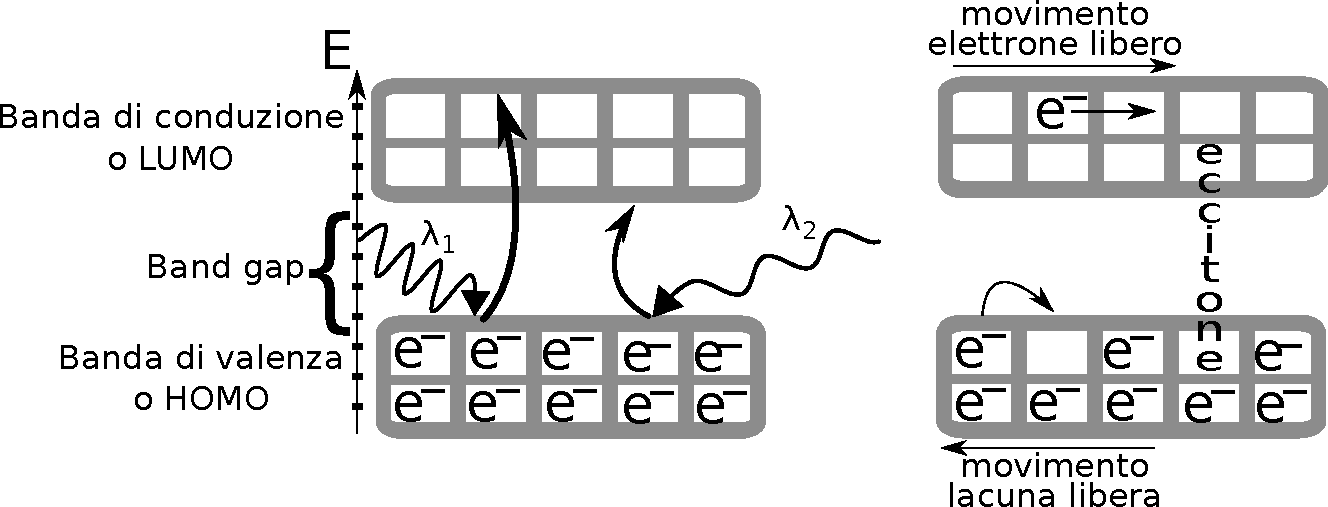
\includegraphics[width=0.9\textwidth]{Immagini_Tesi/semicond-schema2.pdf}}
\end{figure}
\end{frame}
}
%%%%%%%%%%%%%%%%%%%%%%%%%%%%%%%%%%%%%%%%%%%%%%%%%%%%%%%%%%%%%%%%%%%%%%%%%%%%%%%%%%%%%%%%%%%%%%%%%%%%%%%%%%%%%%%%%%%%%%%%%%%%%%%%%%%%

\diapo{Separazione degli eccitoni in cariche all'interfaccia}

\alert{Le coppie eccitoniche possono essere scisse in carica e lacuna per recuperarne l'energia.} 
\begin{columns}
\column{0.66\linewidth}\uncover<2->{
\begin{itemize}
 \item Sono necessari forti campi elettrici come quelli che si formano all'\alert{interfaccia} tra due semiconduttori con livelli energetici diversi.
 \item In assenza di processi di scissione si propagano in semiconduttori organici per non più di 20~nm (massimo cammino eccitonico) dopodiché decadono radiativamente.
\end{itemize}}
\column{0.34\linewidth}
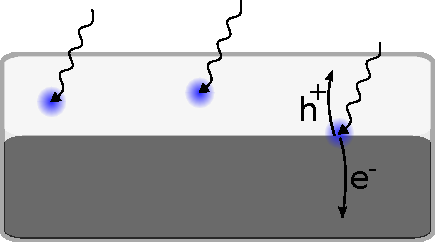
\includegraphics[width=1\textwidth]{Immagini_Tesi/bilayer-eccitoni.pdf}
\end{columns}
\end{frame}

%%%%%%%%%%%%%%%%%%%%%%%%%%%%%%%%%%%%%%%%%%%%%%%%%%%%%%%%%%%%%%%%%%%%%%%%%%%%%%%%%%%%%%%%%%%%%%%%%%%%%%%%%%%%%%%%%%%%%%%%%%%%%%%%%%%%

\subsection{Morfologia con interfaccia distribuita}
\begin{frame}
\frametitle{Morfologia con interfaccia distribuita (1)}
Una tradizionale morfologia con uno strato di polimero ed uno di nanoparticelle (\emph{bilayer}) non presenta sufficiente interfaccia.
 \begin{figure}\centering{
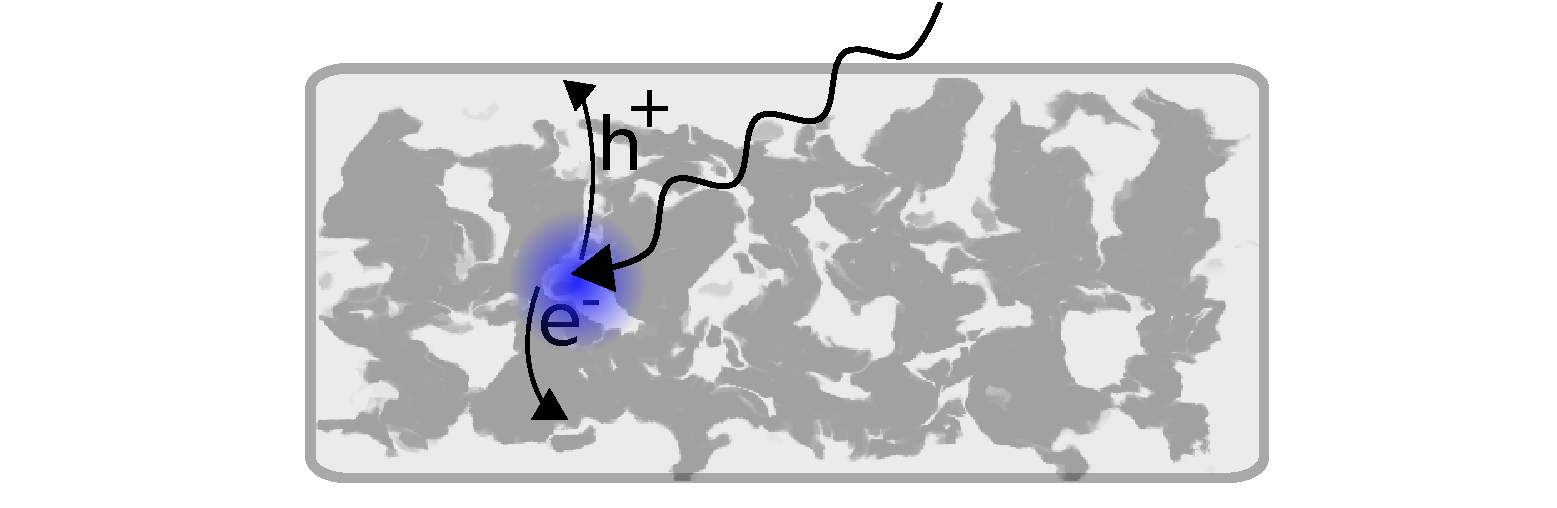
\includegraphics[width=.605\textwidth]{Immagini_Tesi/bulk-heterojunction-eccitoni.pdf}}\end{figure}
Una morfologia con interfaccia distribuita (\emph{bulk heterojunction}) permette di raggiungere efficienze energetiche più elevate.


\end{frame}

%%%%%%%%%%%%%%%%%%%%%%%%%%%%%%%%%%%%%%%%%%%%%%%%%%%%%%%%%%%%%%%%%%%%%%%%%%%%%%%%%%%%%%%%%%%%%%%%%%%%%%%%%%%%%%%%%%%%%%%%%%%%%%%%%%%%
\begin{frame}
\frametitle{Morfologia con interfaccia distribuita (2)}
\framesubtitle{Mantenere la morfologia \emph{bulk heterojunction} con leganti}
\begin{columns}
\column{0.68\linewidth}
\begin{block}{In questo lavoro di tesi:} Si è funzionalizzato un polimero con dei \alert{gruppi~leganti} per aumentare la disperdibilità delle nanoparticelle.\\
Tra le varie possibilità per il posizionamento dei leganti, in questa tesi è stata realizzata l'\alert{ultima in figura}.\end{block}
\column{0.3\linewidth}{\begin{figure}\centering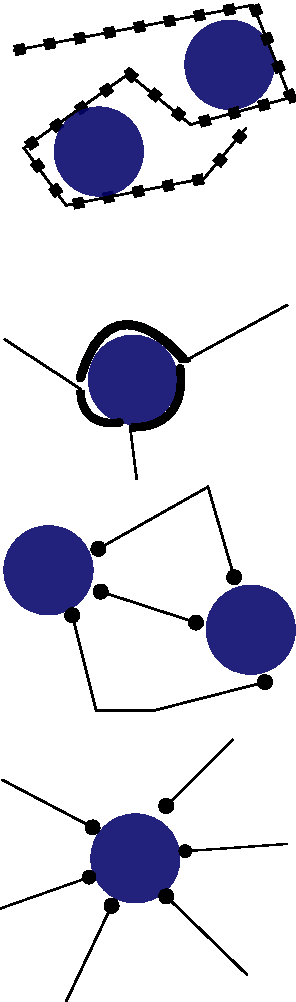
\includegraphics[width=0.5\textwidth]{Immagini_Tesi/leganti-verticale.pdf}\end{figure}}
\end{columns}
\end{frame}
